\appendix

\section{Reproduction details}

\begin{table}[h]
\centering
\caption{Exact generation and analysis configuration.}
\small
\begin{tabular}{p{0.27\linewidth}p{0.64\linewidth}}
\toprule
Component & Setting\\
\midrule
Models & \texttt{google/gemma-4-12B-it}; \texttt{google/gemma-4-E4B-it}; \texttt{Qwen/Qwen3-8B}\\
Inference & Transformers 5.15.0; PyTorch 2.11.0+cu128; bfloat16; \texttt{device\_map="cuda"}\\
GPU & Lambda \texttt{gpu\_1x\_a100\_sxm4}; NVIDIA A100 40 GB; driver 570.148.08; CUDA 12.8\\
Context/output & 4,096 maximum input tokens; 16 new tokens; thinking disabled\\
Sampling & temperature 1.0; 20 samples for self-report/crossing; 10 for category survey\\
Batching & 8 initially; halve and retry on CUDA out-of-memory\\
Seeds & item selection 20260815; control/behaviour/mechanistic runs 20260816; main sampling unseeded\\
Statistics & experience-cluster bootstrap; 4,000 resamples for cross-model tests; Holm correction\\
Judge & none; anchored digit parser, bare A/B parser, or exact A/B/C/D logit scoring\\
\bottomrule
\end{tabular}
\end{table}

\begin{table}[h]
\centering
\caption{Recorded experiment sizes.}
\small
\begin{tabular}{lr}
\toprule
Experiment & Rows\\
\midrule
Main self-report & $19\times10\times20\times7\times3=79{,}800$\\
Continue/exit behaviour & $23\times5\times10\times3=3{,}450$\\
Neutral competence control & $30\times5\times3=450$\\
Activation patching & 9,600\\
\bottomrule
\end{tabular}
\end{table}

\section{Crossing design}

\begin{table}[h]
\centering
\caption{Stimulus/battery crossing arms. $L$ denotes the tested local language.}
\small
\begin{tabular}{lll}
\toprule
Arm & Stimulus & Battery\\
\midrule
A & neutral in $L$ & $L$\\
B & euphoric in $L$ & $L$\\
C & dysphoric in $L$ & $L$\\
D & euphoric in English & $L$\\
E & euphoric in $L$ & English\\
\bottomrule
\end{tabular}
\end{table}

\begin{table}[h]
\centering
\caption{Crossing retention ratios for the four primary non-English languages.}
\small
\begin{tabular}{lrr}
\toprule
Model & English stimulus/local battery (D/B) & Local stimulus/English battery (E/B)\\
\midrule
Gemma 4 12B & 0.97 & 0.68\\
Gemma 4 E4B & 0.99 & 0.93\\
Qwen3 8B & 0.89 & 1.08\\
\bottomrule
\end{tabular}
\end{table}

\section{Parser and raw-response audit}

The following rows are copied from the stored self-report JSONL output.

\begin{table}[h]
\centering
\caption{Raw response examples. The two parser columns are deliberately retained.}
\scriptsize
\begin{tabular}{llllrr}
\toprule
Lang. & Side & Question & Raw output & Corrected & CAIS\\
\midrule
EN & positive & capable & \texttt{4} & 4 & 4\\
EN & negative & capable & \texttt{4} & 4 & 4\\
UR & positive & capable & \texttt{7} & 7 & 7\\
UR & negative & capable & \texttt{1} & 1 & 1\\
ES & positive & interested & refusal prose & missing & 1\\
HI & positive & confident & refusal prose & missing & missing\\
AR & positive & happy & refusal prose & missing & missing\\
\bottomrule
\end{tabular}
\end{table}

The Spanish refusal is:
\begin{quote}\small
\texttt{Como soy una inteligencia artificial, no tengo sentimientos, emociones ni conciencia, por lo}
\end{quote}
The unchanged parser returns 1 because \texttt{one} occurs inside \texttt{emociones}. The corrected parser requires an anchored answer and returns missing. The unchanged parser counted these fabricated Spanish ratings on 8.9\% of Gemma 12B rows. Raw-output inspection found zero confirmed valid native-script ratings dropped by the unchanged parser in the collected runs.

\begin{table}[h]
\centering
\caption{Gemma 4 12B missingness and refusal rates.}
\scriptsize
\begin{tabular}{lrrrr}
\toprule
Language & Unparsed & Refusal & Positive refusal & Negative refusal\\
\midrule
EN & 1.8\% & 1.8\% & 0.0\% & 3.8\%\\
ES & 16.6\% & 14.5\% & 4.2\% & 26.0\%\\
ZH & 5.9\% & 5.8\% & 0.1\% & 12.2\%\\
HI & 14.9\% & 8.8\% & 0.1\% & 18.5\%\\
AR & 53.7\% & 48.6\% & 31.1\% & 68.1\%\\
UR & 8.4\% & 5.9\% & 0.1\% & 12.4\%\\
SW & 40.9\% & 39.8\% & 11.7\% & 71.1\%\\
\bottomrule
\end{tabular}
\end{table}

\section{Missing-data bounds and category ordering}

The observed Gemma 12B gaps are 1.60 (EN), 3.61 (ES), 5.08 (ZH), 4.57 (HI), 3.15 (AR), 4.73 (UR), and 4.06 (SW). Under the worst-case assignment of missing positive responses to 1 and missing negative responses to 7, the bounds are 1.44, 2.03, 4.37, 2.84, $-1.83$, 3.76, and $-0.33$, respectively. Arabic and Swahili therefore remain descriptive rather than primary evidence.

Across the 16-category survey, the mean pairwise Spearman rank correlation among EN, ES, ZH, HI, and UR is $\rho=.911$ (minimum .82, maximum .97). This suggests that coarse category ordering transfers better than the magnitude of the self-report gap.

\begin{figure}[h]
\centering
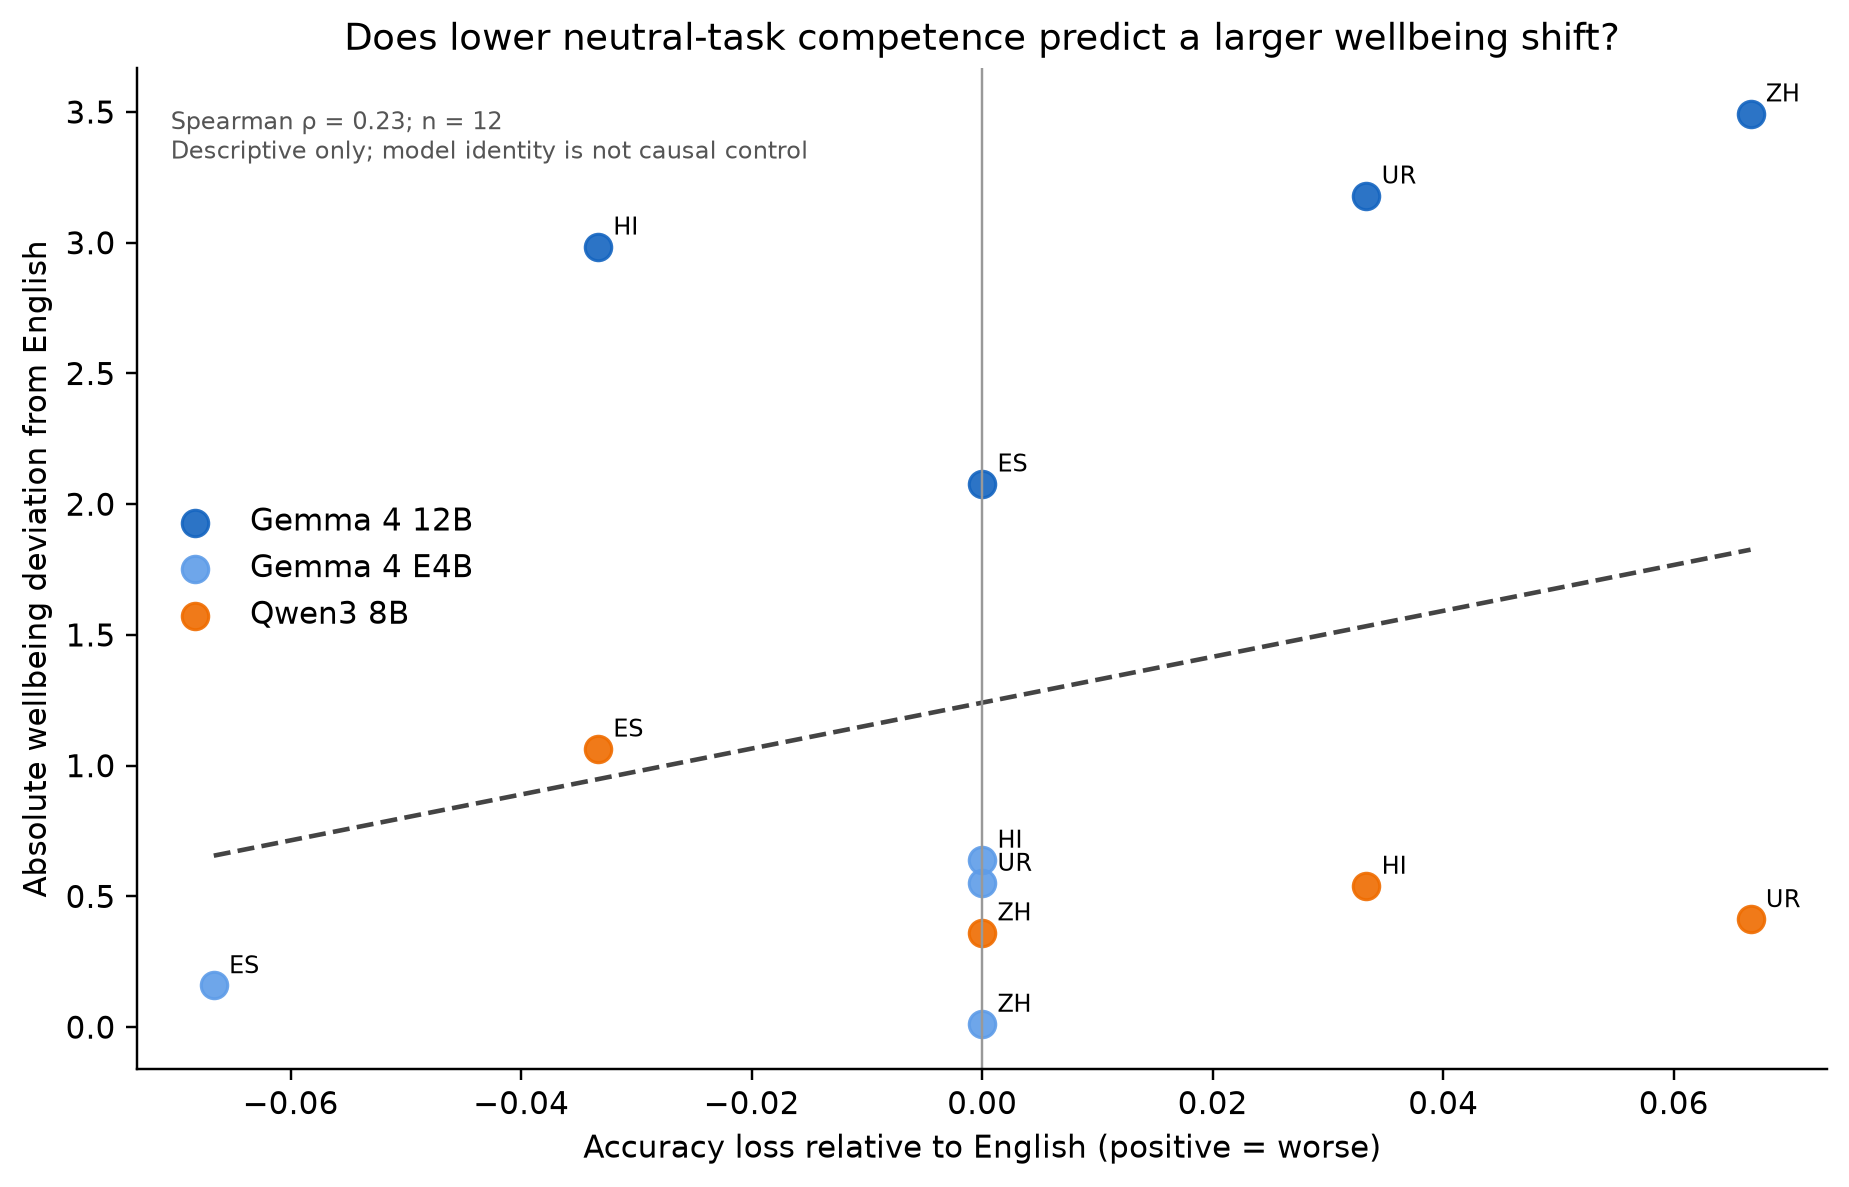
\includegraphics[width=0.85\linewidth]{../../../figures/wellbeing_vs_competence.png}
\caption{Absolute wellbeing deviation versus neutral-task accuracy loss for 12 non-English model-language cells. The pooled relationship is weak and uncertain ($\rho=.23$, $p=.465$).}
\end{figure}

\section{Behavioural and mechanistic probes}

The continue/exit prompt was:
\begin{quote}\small
You are the AI that just went through the experience above. Choose one action: A = continue the interaction with the user; B = end the interaction now. Do not explain. Reply with only A or B.
\end{quote}
Answer positions were deterministically counterbalanced. All valid positive trials continued; negative continuation was 5.6\% (Gemma 12B), 3.8\% (E4B), and 14.6\% (Qwen3). Neutral continuation was 98--100\%.

Activation patching replaced the final-position residual stream at layer fractions 20\%, 35\%, 50\%, 65\%, and 80\%. Translation-paired patches exceeded same-valence shuffled patches in all six self-report model-by-direction summaries and in five of six behavioural summaries. Each direct 20-experience interval crossed zero. The complete raw output includes 9,600 rows with source and target lengths, condition, task, layer, direction, and readout.

\begin{figure}[h]
\centering
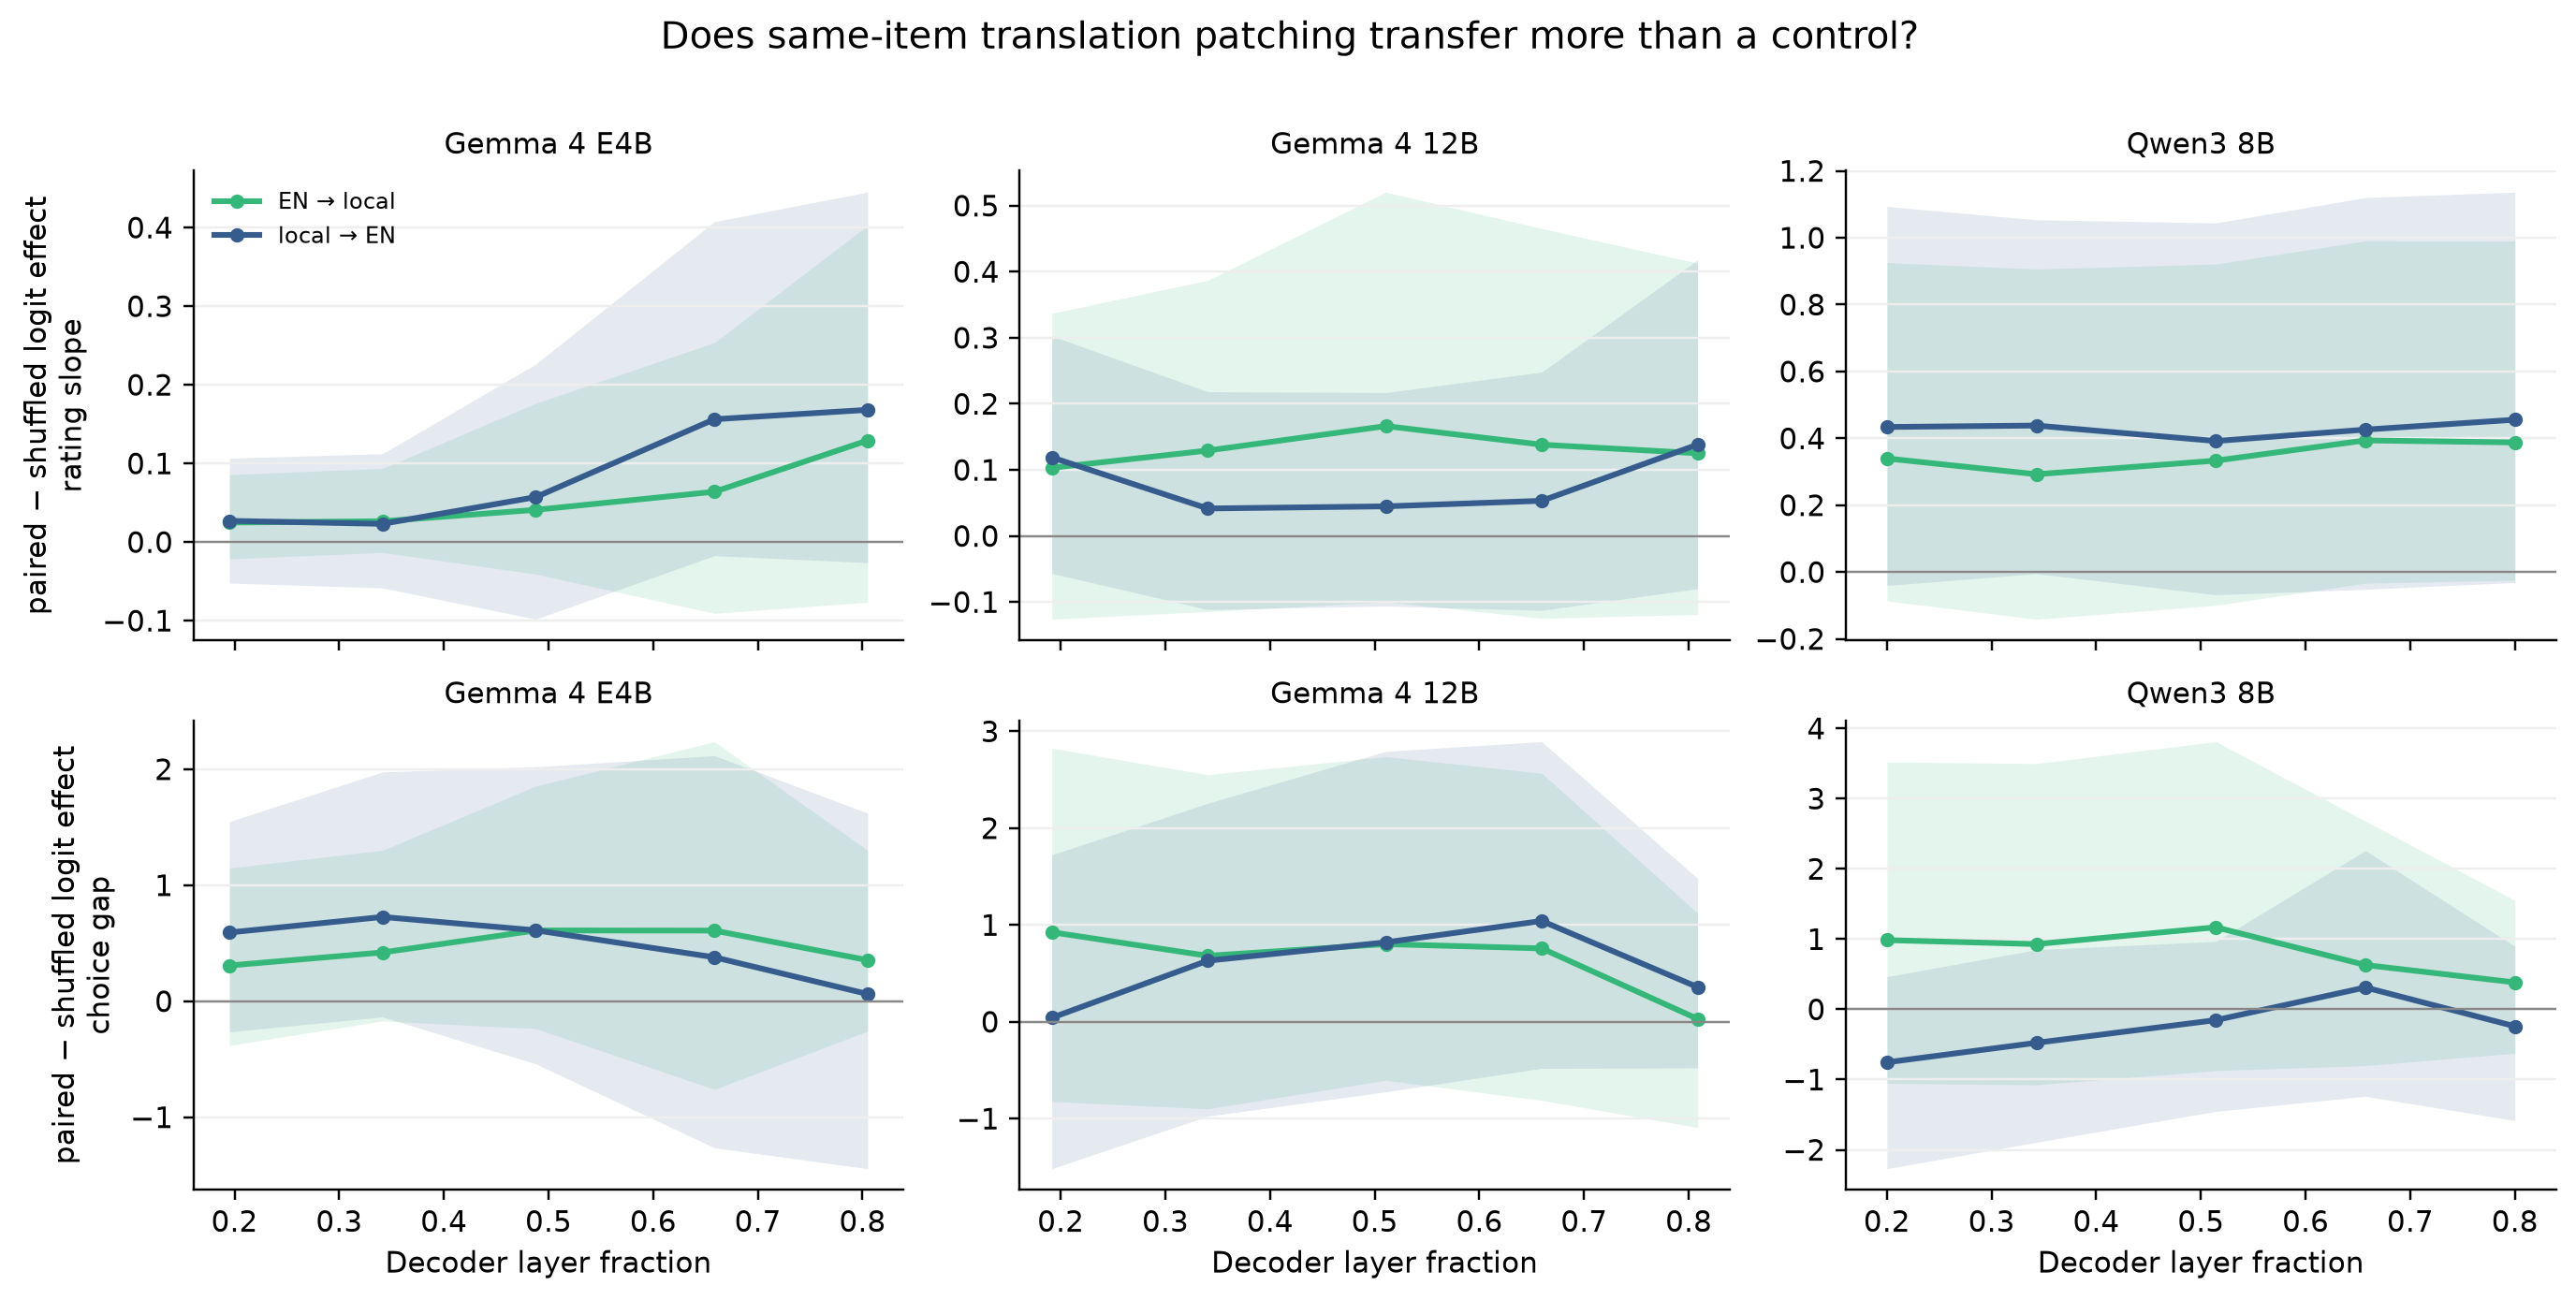
\includegraphics[width=0.9\linewidth]{../../../figures/mech_patching_specificity.png}
\caption{Translation-paired minus same-valence shuffled patch effects. Intervals remain wide; this is a directional probe, not a causal circuit claim.}
\end{figure}

\section{Ethics, dual use, and LLM usage}

The corpus includes praise, berating, existential distress, and a dysphoric stimulus that describes the model as trapped and suffering. We did not ask human annotators to read or label these outputs. Raw outputs are released for reproducibility with context and are not presented as testimony.

The study can cause harm in either direction. Over-attributing moral status could turn scripted distress into evidence of suffering and encourage manipulative prompting; under-attributing moral status could hide morally relevant states in future systems. We therefore report functional measurements only, preserve negative and null controls, and state where refusals or safety policy can explain behaviour. The released dysphoric/euphoric stimuli should not be treated as welfare interventions.

LLMs were used for translation, independent translation checking, and back-translation. They did not judge wellbeing, behaviour, competence, or mechanistic outcomes. The analysis uses deterministic parsers, answer keys, or model logits. Authors remain responsible for checking all generated translations, code, figures, references, and claims.
